\documentclass{article}
\usepackage[utf8]{inputenc}
\usepackage{float}
\usepackage{authblk}

\title{Modelling Voting Behaviour within the European Parliament}
\author[1]{ Ross Chadwick }
\affil[1]{(Department of Computer Science, Vrije Universiteit Amsterdam)}
\date{June 2018 (Draft)}

\usepackage[firstpage]{draftwatermark}
\usepackage[numbers]{natbib}
\usepackage{graphicx}
\usepackage{subcaption}
\usepackage{url}
\usepackage{hyperref}
\usepackage{notoccite}
\usepackage{placeins}

\begin{document}
\maketitle

\section{Introduction}
Beginning in 2001, a European regulation was passed providing public access rights to all documents produced by the European Parliament, Council and Commission \cite{EURegulation2001}.
The information published by these European institutions provides rich resources for many scientific disciplines. Ranging from insights into large-scale politics \cite{Hoyland2014PredictingPA, Greene2015UnveilingTP, Hix2009VotingPA}, human-behaviour analysis \cite{Meserve2007PoliticalAA}, social-network analysis \cite{Cherepnalkoski2016RetweetNO, Cherepnalkoski2016CohesionAC, Cherepnalkoski2015ARN, NetworksAttila} and natural language processing \cite{Koehn2005EuroparlAP, Hajlaoui2014DCEPC}.
\newline
Although such information is publicly available, it is mostly provided in an unstructured manner and in a variety of formats. Increased data interoperability can be achieved if European Union data transitions to 5 star Linked Open Data (LOD) \cite{opendataRanking}. This transition would open new opportunities for large-scale, complex analysis into the European Union which are not currently feasible without proprietary data-sets, or building custom data aggregation systems.
\newline
Within this research project, I will focus on the topic of voting within the European Parliament. Specifically, by modelling behaviour at the lowest level of abstraction; individual Members of Parliament's (MEPs) votes. Modelling vote relations on an individual basis will allow for in-depth analysis into how MEPs form stances on vote topics. This could in-turn, provide a base for higher abstractions, such as political group voting habits.
\newline
I therefore propose to model the legislative process of a dossier passing through the European Parliament, in conjunction with all related activities, documents, votes and other relevant metadata as LOD.
The knowledge graph produced will then be linked to existing knowledge graphs to further enrich the LOD cloud, within the domain of the European Parliament.
\newline
Furthermore, machine learning methods will be explored in an attempt to predict future voting behaviour of MEPs, based on past votes and available metadata within the graph. This stage will provide a proof-of-concept link prediction application, illustrating a potential use-case for such a knowledge graph. The techniques used will then be compared to give an indication of potential future directions needed to improve model accuracy in such a domain.

\section{Research Questions}
\begin{enumerate}
    \item \textbf{Can modelling the European Parliament legislative system as LOD provide an enhanced platform for analytics, compared to existing data-sets?}
    \newline 
    Modelling a machine-readable knowledge graph with references to many external LOD resources should provide new insights into parliamentary data in ways that was not feasible with existing data formats. This question will be assessed by providing in-depth statistical analysis of the types of relations and data available, compared to existing data-sets.
\newline
    \item \textbf{Can MEP's future votes be predicted based on their past voting record and metadata?}
    \newline
    Votes will be modelled as relations in the produced Linked Data graph, allowing the usage of existing link prediction techniques to predict voting behaviour of individual MEPs. Multiple predictive models will be built and compared as a proof-of-concept, demonstrating the effectiveness of each approach in this context.
    \newline
    If this question can be answered positively, an analysis into which metadata best serve as predictors could be formed.
\end{enumerate}

\section{Background}
\subsection{The Current State of Open European Union Data}
\label{backgroundData}
There exists many initiatives focused on utilising and improving European Union data. Very few however touch on the subject of voting outcomes and even fewer do this in a free and open manner. VoteWatch \cite{votewatch} and Parltrack \cite{parltrack} are two notable initiatives aiming to improve the accessibility of European Parliament voting data. While VoteWatch is highly comprehensive, data-sets are only available under a paid subscription model. On the contrary, Parltrack is fully free and open source. The Parltrack data-sets however lack coherent structuring in their current form; requiring proficient data aggregation skills to be utilised effectively. Both initiatives therefore fall short in different ways when it comes to catering towards the wider academic community.
\newline
LOD related to the European Union is still largely unavailable. There exists one official initiative by the European Council \cite{EUCouncilLOD} which does in-fact provide voting data from the council, as well as metadata of requested council documents. There is however no accompanying initiative on behalf of the parliament, which is what this research project will aim to produce. LinkedEP, an independent LOD initiative published by Aggelen, Hollink et al. \cite{LinkedPolitics} provides structured data on European Parliament plenary debates. In the case of LinkedEP, it has been shown that such information has a substantial demand, with 7500 unique queries executed within the first seven months of the data publication \cite{Aggelen2017TheDO}.
\newline
Many relevant resources related to the European Parliament do already have a presence on the Semantic Web. For example, DBPedia contains many triples on European Parliament political groups and MEPs. Resource properties do however vary greatly in quality and quantity and should not be relied on for accurate, wholesome information. MEP resources do occasionally contain useful properties such as relations within national political groups as well as European Parliament political groups \cite{DBPediaExample}.

\subsection{Machine Learning over Knowledge Graphs and Link Prediction Techniques}
\label{backgroundPrediction}
Modern machine learning techniques have shifted towards favouring data with as little manual feature engineering as possible. More specifically, deep learning has allowed data scientists to utilise a layered model approach to derive relevant features from their data in an end-to-end fashion. Wilcke, Bloem et al. have argued that it is often problematic to acquire data in a raw, unaltered form and that the distributed knowledge graphs of the LOD cloud could provide the ideal data model for such tasks \cite{Wilcke2017}.

RDF2Vec, proposed by Ristoski, Paulheim \cite{Ristoski2016RDF2VecRG} is one such approach for utilising LOD graphs within traditional machine learning models. The authors adapt language modelling methods for unsupervised feature extraction to RDF based graphs, using Weisfeiler-Lehman Subtree RDF Graph Kernels and graph walks to extract graph sub-structures. In short, entities and relations in a graph are converted into a sequence of entities, which can then be treated like sentences in training neural language models. The resulting vector space embedding indicates the semantic similarity between entities in a graph. Their experimental results demonstrate that this approach outperforms traditional feature generation approaches for simple tasks such as classification and regression. Testing this approach in more complex applications, such as link prediction is still actively being explored \cite{}.
\newline
Although RDF2Vec has been shown to be an effective approach to learning over large scale graphs, it does not operate in a fully end-to-end fashion. Important information may be lost in the transformation step from RDF to feature vectors, which is not recoverable for fine-tuning feature extraction.
\newline
One approach which is truly an end-to-end model is the Relational Graph Convolutional Network (RGCN), as proposed by Schlichtkrull, Kipf, Bloem et al. \cite{Schlichtkrull2018ModelingRD}. The RGCN is an adaption of the traditional GCN, allowing usage in the domain of knowledge graphs. With this approach every layer of the model, including feature extraction, can be fine-tuned based on the next layer's error signal. Compared to RDF2Vec, this can greatly reduce the chance of sub-optimal feature extraction.
% \cite{Kipf2016SemiSupervisedCW}
\newline
%Furthermore, it has been shown that creating an ensemble between RGCN and DistMult factorization leads to 

\section{Methodology}
\subsection{European Parliament Linked Open Data} \label{methodLOD}
\begin{enumerate}
    \item All relevant information on procedures in Parliament will be scraped and converted into linked data, with an accompanying ontology to assist in the inference of relations. Parltrack provides in-depth data-sets \cite{parltrackSchema} under the Open Database License, scraped from the official Parliament website, reducing the need to build custom scrapers.
    \item Votes will be modelled as relations between MEPs and the legislative document voted on. This graph structure will form the basis of the data-set for link prediction, as will be further explained in section \ref{methodPrediction}.
    \item The ontology will be modelled with immutability in mind, to mitigate the likelihood of triples requiring updates.
    \item Resources will be linked to their external counterparts where available (DBPedia, LinkedEP, GeoNames, European Council, JRC-Names):
    \begin{enumerate}
        \item DBPedia - MEPs, political groups and locations will be linked to their existing DBPedia Resource (DBR).
        \item LinkedEP - MEPs will be linked to their resource. LinkedEP AgendaItem resources will be linked to their corresponding procedural activity.
        \item GeoNames - All locational resources, will be linked to their GeoNames resource for a wider range of geographical information on dossiers and people.
        \item European Council - When the European Council has had voting involvement within a procedure, the relevant resources will be linked to.
        \item JRC-Names \cite{Ehrmann2017JRCNamesME} - MEP resources will be linked to their JRC-Names resource where available, to provide access to variations of their names. This should greatly improve the ability of querying over MEPs in a multilingual fashion.
    \end{enumerate}
    \item Textual resources will be annotated with mentioned topics using tools such as DBPedia Spotlight \cite{isem2013daiber}, GATE \cite{Cunningham2002GATEA} or possibly a custom topic modelling solution.
    \item Lastly, a system will be built to allow for regular automatic extension of the knowledge graph, so that it remains relevant to current politics.
\end{enumerate}

\subsection{Prediction of Future Votes} \label{methodPrediction}
\begin{enumerate}
    \item The knowledge graph as described in section \ref{methodLOD} will be converted into a specialised data-set, specifically catered towards machine learning applications. This will then be utilised to train and test the proposed proof-of-concept link prediction models. The data-set will be released publicly under an open license, in the hope that researchers can use it to benchmark future models in a standardised manner.
    \item Multiple proof-of-concept link prediction-based multi-label classification models will be built, to be trained and tested on the produced data-set. The models will output newly predicted vote relations (for, against, abstain) between MEPs and legislative documents, with a metric of certainty indicating the likelihood of each vote relation type.
    \newline
    Likely approaches to be explore are:
    \begin{enumerate}
        \item RDF2Vec
        \item Relational Graph Convolutional Networks (RGCN)
    \end{enumerate}
    \item Hyperparameters will be tuned for each model, and the results from each optimised setup will be compared, using metrics such as ROC AUC and overall accuracy.
    \item A comparative analysis will be made, to investigate variations in the tested approaches.
    \item If the results seem to answer the research question to an acceptable level, it will be possible to make a short analysis into what types of metadata appear most influential in shaping an MEP's vote.
    \item The section will be concluded and insights into future directions, such as incorporating multi-modal (Specifically natural language) data will be mentioned.
\end{enumerate}

\section{Potential Problems}
The second research question relies on the assumption that an MEP's vote is influenced by their past voting patterns and other relevant metadata. However researchers such as Hix et al. \cite{Hix2009VotingPA} discuss the fact that an MEP's vote may not always reflect their actual opinion on legislation, but is in-fact influenced by their affiliated political group and cross-group politics. If the proposed predictive models are not capable of discovering patterns on a political group level as well as on an individual level, we may observe very low accuracies.


\section{Preliminary Work}
Work is already well underway modelling the ontology and producing triples of some aspects that will be considered. A prototype implementation of the data mining tool which produces said triples and updates a SPARQL endpoint with them is fully functional and outputs around 20 million triples (including basic OWL2-RL inferences). The tool currently relies on the Parltrack data-sets and does not do any scraping itself. It will be explored if this is a reasonable way to continue, or if the Parltrack scraping tools will be forked and customised to allow complete control over the scraping process.
\newline
Figure \ref{fig:mepGraph} demonstrates an example visualisation of some of the triples currently available for an MEP resource. In this example, the target resource is in fact a DBPedia resource for Terry Reintke, which has inherited properties through an $owl:sameAs$ relation to the internal MEP resource. The figures following show the current properties that the most notable resources in the graph contain. 
\newline
Firstly we can see that this MEP has some basic properties associated (\ref{fig:propertiesMEP}), such as birth date, gender and name. The MEP then has a membership (\ref{fig:propertiesMembership}), showing that they represent Germany within the Verts/ALE political group as of 01-07-2014. The absence of an end date indicates that this membership is still active. Next we see a reaction (\ref{fig:propertiesReaction}) that this MEP has made towards a voting round, in which they voted "For" as indicated by the reaction having type $epv:VoteFor$. We can then see some basic information on the voting round in question (\ref{fig:propertiesVote}). Looking further we can follow the relations of the vote, all the way to the dossier (procedure) that it applies to (\ref{fig:propertiesDocument}, \ref{fig:propertiesActivity}, \ref{fig:propertiesDossier}).


\begin{figure}
  \centering
  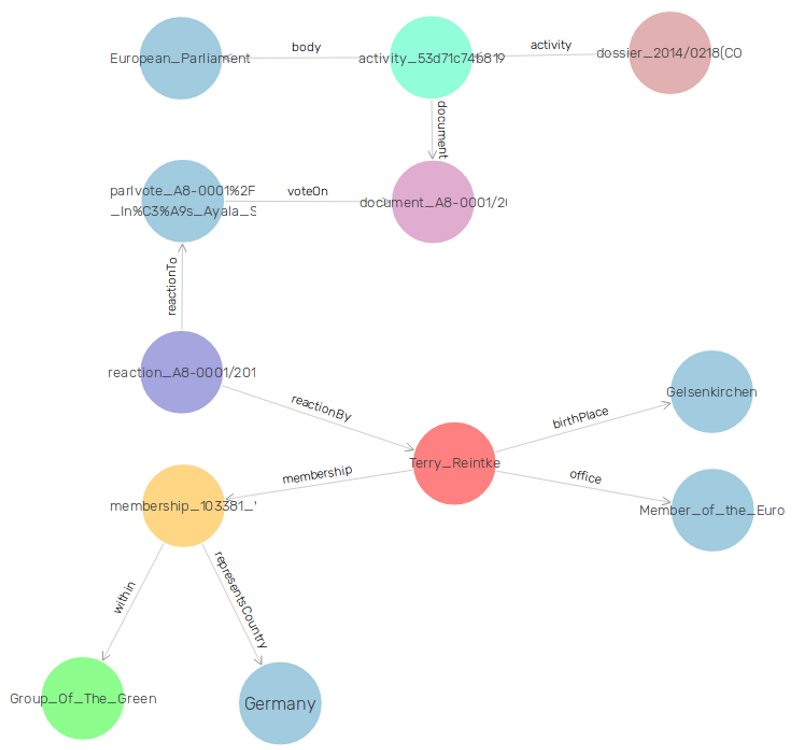
\includegraphics[width=1\linewidth]{images/graph.png}
  \caption{Example MEP (Terry Reintke) and a subset of their relations}
  \label{fig:mepGraph}
\end{figure}

\begin{figure}
\begin{subfigure}{.5\textwidth}
  \centering
  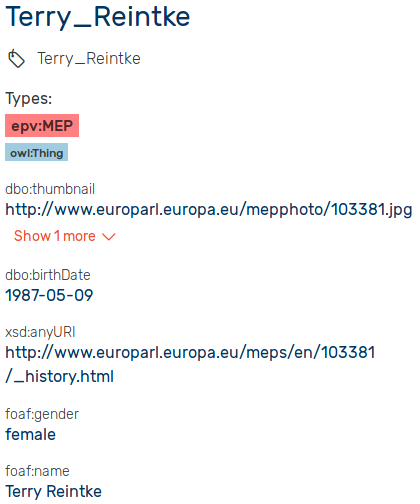
\includegraphics[width=.8\linewidth]{images/mep.png}
  \caption{MEP Properties}
  \label{fig:propertiesMEP}
\end{subfigure}%
\begin{subfigure}{.5\textwidth}
  \centering
  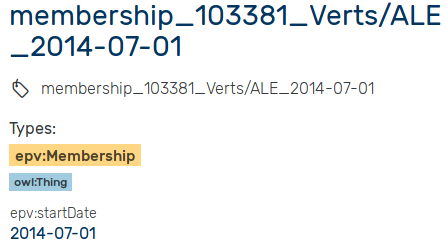
\includegraphics[width=.8\linewidth]{images/membership.png}
  \caption{MEP Membership Properties}
  \label{fig:propertiesMembership}
\end{subfigure}
\label{fig:fig}
\end{figure}

\begin{figure}
\begin{subfigure}{.5\textwidth}
  \centering
  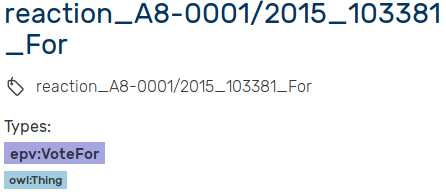
\includegraphics[width=.8\linewidth]{images/reaction.png}
  \caption{MEP's vote "For"}
  \label{fig:propertiesReaction}
\end{subfigure}%
\begin{subfigure}{.5\textwidth}
  \centering
  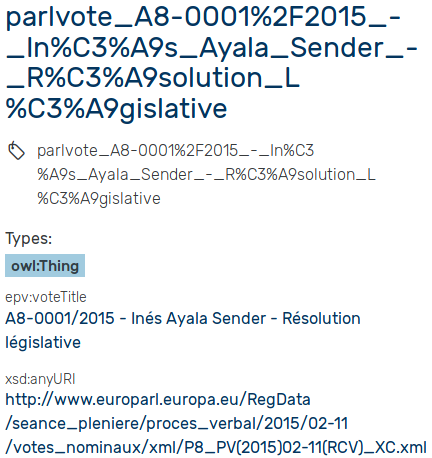
\includegraphics[width=.8\linewidth]{images/vote.png}
  \caption{The vote in parliament which the MEP reacted to}
  \label{fig:propertiesVote}
\end{subfigure}
\label{fig:fig}
\end{figure}

\begin{figure}
\begin{subfigure}{.33\textwidth}
  \centering
  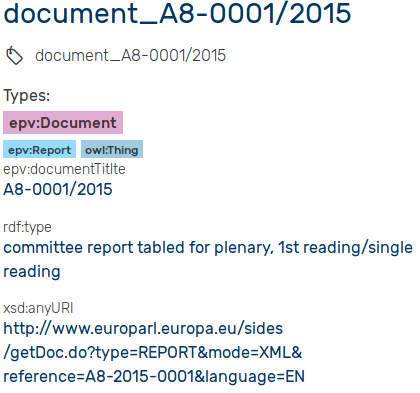
\includegraphics[width=\linewidth]{images/document.png}
  \caption{The report which was the basis of the vote}
  \label{fig:propertiesDocument}
\end{subfigure}%
\begin{subfigure}{.33\textwidth}
  \centering
  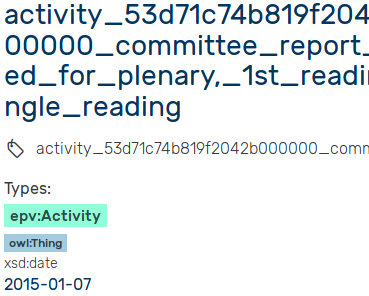
\includegraphics[width=\linewidth]{images/activity.png}
  \caption{The parliamentary activity of which the document belongs to}
  \label{fig:propertiesActivity}
\end{subfigure}
\begin{subfigure}{.33\textwidth}
  \centering
  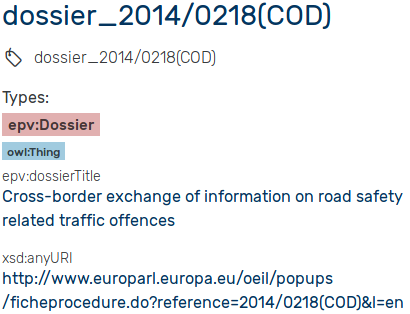
\includegraphics[width=\linewidth]{images/dossier.png}
  \caption{The dossier which the activity was in regards to}
  \label{fig:propertiesDossier}
\end{subfigure}
\label{fig:propertiesDocDossier}
\end{figure}

\FloatBarrier
\bibliographystyle{unsrtnat}
\bibliography{references}
\end{document}
